\section{Machine Learning Applications for HMM}
\label{sec:ml}

% introducere in invatare automata + categorisire probleme
\subsection{Machine Learning}
\label{sec:hmm_in_ml}

\begin{frame}
  \frametitle{What is Machine Learning?}
  \begin{block}{Machine Learning}
    A computer program is said to learn from experience $E$ with
    respect to some class of tasks $T$ and performance measure $P$, if
    its performance at tasks in $T$, as measured by $P$, improves with
    experience $E$.
  \end{block}
\end{frame}

\begin{frame}
  \frametitle{Machine Learning Applications}
  \begin{itemize}
  \item Computer Vision: Google Car
  \item Machine Translation
  \item Speech Recognition
  \item Recommender Systems
  \item Intelligent Advertising
  \end{itemize}
\end{frame}

% aplicatii specifice hmm-urilor de ce am ales hmm-urile
\subsection{Where do HMMs fit into Machine Learning?}
\label{sec:apps}

\begin{frame}
  \frametitle{Machine Learning Classification}
  Types of Machine Learning Problems
  \begin{columns}
    \column{0.7\textwidth}
    \begin{itemize}
    \item Regression
    \item Classification
    \item Reinforcement Learning
    \end{itemize}
    \begin{itemize}
    \item supervised learning (eg. ..)
    \item unsupervised
    \end{itemize}
    \column{0.3\textwidth}
    \includegraphics[width=\textwidth]{graphics/ml.pdf}
  \end{columns}
\end{frame}

%% aici facem tranzitie de la problema generala de ML
%% la probleme cu secvente temporale, markov stuff, dbn shit
%% adica HMM-uri :))

%% Markov models, Dynamic Bayesian Networks
\begin{frame}
  \frametitle{Sequence / Temporal problems (I)}
  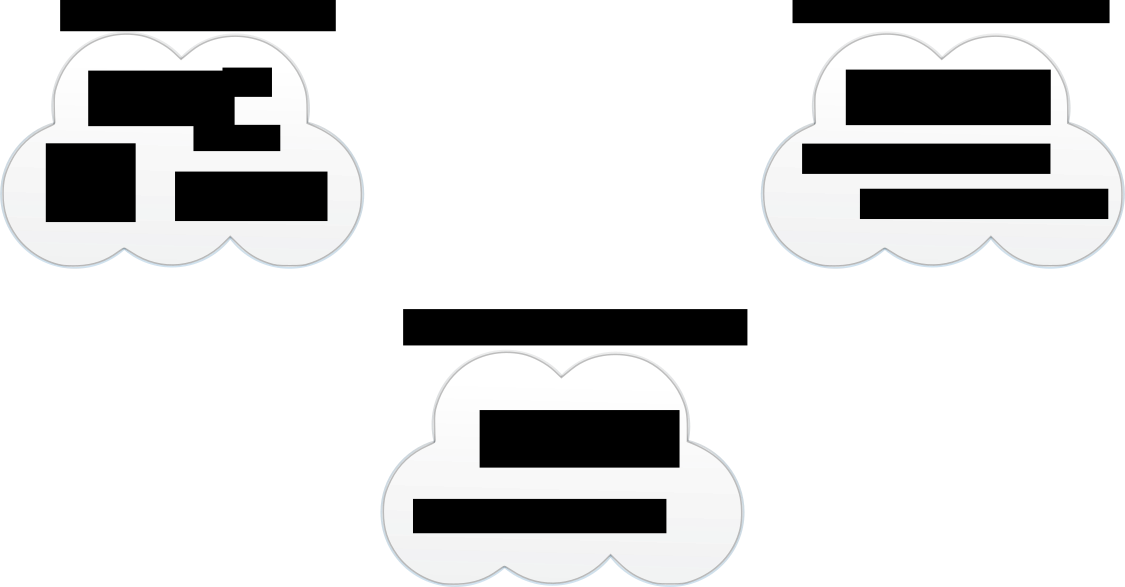
\includegraphics[width=\textwidth]{images/time_series_problems_1.pdf}
\end{frame}

\begin{frame}
  \frametitle{Sequence / Temporal problems (II)}
  \includegraphics[width=\textwidth]{images/time_series_problems_2.pdf}
  %Koller and Frideman au scris in \cite{KollerFriedman09}
  % temporal sequences
  % DBN for ts
  % HMM as a special case of DBN
\end{frame}


% descrierea a ceea ce inseamna Probabilistic Reasoning over Time (capitol 15.2 AI a modern approach)
% 	- states and observations
\begin{frame}[t]
  \frametitle{Probabilistic Reasoning over Time - Models}
	Consider some of the previously presented problems ...
	\vspace*{0.5em}
	\pause	
	
	How do we model such dynamic situations? 
	\vspace*{1em}
	\pause	
	
	\textbf{States and Observations}
	\begin{itemize}
		\item The process of change is viewed as a series of \alert{time slices (snapshots)}
		\item Each time slice contains a set of random variables
    	\begin{itemize}
	    	\item $\mathbf{O}_t$ - set of all \alert{\emph{observable}} evidence variables at time \emph{t}
			\item $\mathbf{Q}_t$ - set of all \alert{\emph{unobservable / hidden}} state variables at time \emph{t}
		\end{itemize}
	\end{itemize}
\end{frame}

%	- stationary process, Markov assumption, Sensor model
\begin{frame}[t]
  \frametitle{Probabilistic Reasoning over Time - Assumptions}
	Consider some of the previously presented problems ...
	\vspace*{0.5em}
	\pause	
	
	What \alert{assumptions} (if any) do we make?
	\pause	
	
	\begin{block}{Stationary Process}
		The process of change is governed by laws \alert{that do not themselves change over time}.\\
		\alert{Implication:} we need to specify conditional distributions only for the variables within a \emph{representative} timeslice.
	\end{block}
	
	\pause	
	
	\begin{block}{Markov Assumption}
		The current state in a process of change depends only on a \alert{finite history} of previous states.
		\\
		\alert{Implication:} there is a \alert{bounded} number of ``parents'' for the variables in each time 
		slice.\\
		$\mathbf{P}(\mathbf{Q}_t \vert \mathbf{Q}_{1:t-1}) = \mathbf{P}(\mathbf{Q}_t \vert \mathbf{Q}_{t-1})$
		\hspace*{1em}
		$\mathbf{P}(\mathbf{O}_t \vert \mathbf{Q}_{1:t}, \mathbf{Q}_{1:t-1}) = \mathbf{P}(\mathbf{O}_t \vert \mathbf{Q}_t)$
	\end{block}
  
\end{frame}

%	- inference in temporal models
%		- filtering
%		- prediction
%		- smoothing (hindsight)
%		- most likely explanation
%		- model learning
\begin{frame}
  \frametitle{Probabilistic Reasoning over Time - Inference}
	What are the basic inference tasks that must be solved?
	\pause	
	
	\begin{block}{Filtering (monitoring)}
		The task of computing the \alert{belief state} - the posterior distribution over the 
		\alert{current state}, given all evidence to date.\\
		$\mathbf{P}(\mathbf{Q}_t \vert \mathbf{o}_{1:t})$
	\end{block}
	\pause
	
	\begin{block}{Evaluation (likelihood)}
		The task of computing the \alert{likelihood} of the evidence up to present.\\
		$\mathbf{P}(\mathbf{o}_{1:t})$
	\end{block}  
\end{frame}

\begin{frame}
  \frametitle{Probabilistic Reasoning over Time - Inference}
	\begin{block}{Prediction}
		The task of computing the posterior distribution over the \alert{future state}, 
		given all evidence to date.\\
		$\mathbf{P}(\mathbf{Q}_{t+k} \vert \mathbf{o}_{1:t})$, for some $k > 0$
	\end{block}
	\pause
	
	\begin{block}{Smoothing (hindsight)}
		The task of computing the posterior distribution over a \alert{past state}, 
		given all evidence to the present.\\
		$\mathbf{P}(\mathbf{Q}_k \vert \mathbf{o}_{1:t})$, for some $1 \le k < t$\\
		Provides a better estimate of the state than was available at the time.
	\end{block}
\end{frame}

\begin{frame}
  \frametitle{Probabilistic Reasoning over Time - Inference}
	\begin{block}{Most likely explanation}
		Given a \emph{sequence of observations}, find the \alert{sequence of states} that is 
		\alert{most likely} to have generated those observations.
		$argmax_{q_{1:t}}$ $\mathbf{P}(\mathbf{q}_{t+k} \vert \mathbf{o}_{1:t})$, for some $k > 0$
	\end{block}
	\pause
	
	\begin{block}{Learning}
		Given a set of \emph{observation sequences}, find a method to learn the \alert{transition} 
		(e.g. $\mathbf{P}(\mathbf{q}_{t+1} = s_j \vert \mathbf{q}_t = s_i)$, $1 \le i,j < N$) and \alert{sensor} ($\mathbf{P}(\mathbf{o}_t \vert \mathbf{q}_t)$) 
		\alert{models} from the observations.
	\end{block}
\end{frame}

\begin{frame}[t]
    \frametitle{Probabilistic Reasoning over Time - Known Methods}
    
  	\begin{block}{Dynamic Bayesian Networks (DBN)}
  		A DBN is Bayesian network that represents a temporal probability model.
  	\end{block}
  	
  	\begin{figure}
  		\centering
  		
		\begin{subfigure}[b]{0.18\textwidth}
			\centering
  			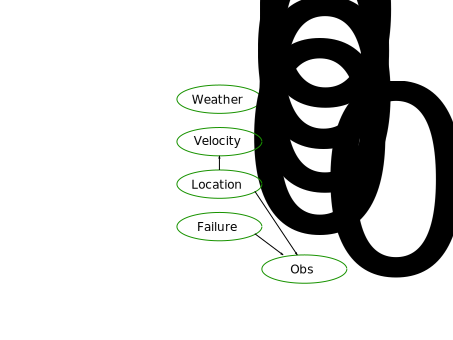
\includegraphics[width=\textwidth]{dbn-vehicle/zero.pdf}
  			\caption{\tiny{the 2-time-slice Bayesian Network}}
  			\label{fig:2TBN}
  		\end{subfigure}
  		\begin{subfigure}[b]{0.33\textwidth}
			\centering
			\includegraphics[width=\textwidth]{dbn-vehicle/transition.pdf}
  			\caption{\tiny{the time 0 network}}
  			\label{fig:zeroDBN}
  		\end{subfigure}
  		\begin{subfigure}[b]{0.39\textwidth}
			\centering
			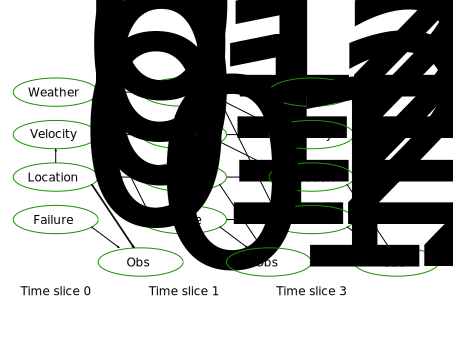
\includegraphics[width=\textwidth]{dbn-vehicle/unrolled.pdf} 
  			\caption{\tiny{unrolled DBN over 3 time slices}}
  			\label{fig:unrolledDBN}
  		\end{subfigure}
  		\caption{\tiny{A highly simplified DBN for monitoring a vehicle \parencite{KollerFriedman09}}}
  		\label{fig:DBN}
  	\end{figure}
  	
  	Applied in problems like: object tracking, human activity recognition, protein sequencing etc.
\end{frame}


\begin{frame}[t]
    \frametitle{Probabilistic Reasoning over Time - Known Methods}
  
  \begin{block}{Kalman Filters (Linear Dynamical Systems)}
  	A temporal model of one or more real-valued variables that \alert{evolve linearly} over time, with some 
  	\alert{Gaussian noise}.
  \end{block}
  
  \begin{columns}[T]
  	\column{0.4\textwidth}
  	\begin{figure}
  		\centering
  		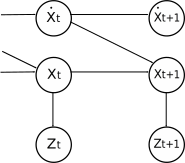
\includegraphics[height=0.35\textheight]{images/kalman_filter_simple.pdf}
  		\caption{\tiny{BN structure for a linear dynamical system with position $X_t$, 
  		velocity $\dot{X}_t$, and position measurement $Z_t$}}
  	\end{figure}
	  
  	\column{0.6\textwidth}
  	\begin{itemize}
  	\item \footnotesize{can be viewed as DBNs where all variables are continuous and all dependencies are 
  		linear gaussian}
  	\item \footnotesize{wide application in \textbf{object tracking}}
  \end{itemize}
  \end{columns}
  
\end{frame}

\begin{frame}[t]
    \frametitle{Probabilistic Reasoning over Time - Known Methods}
  
  \begin{block}{Hidden Markov Models (HMM)}
  	An HMM is a temporal probabilistic model in which the state of the process is described by 
  	\alert{a single discrete} random variable. The possible values of the variable are the possible states of the world.
  \end{block}
  
  \vspace*{1em}
  
  Used successfully in applications like:
  \begin{itemize}
  	\item Handwriting Recognition
  	\item Gesture Recognition
  	\item Speech Recognition
  	\item Part-of-Speech Tagging
  	\item DNA Sequencing
  \end{itemize}
\end{frame}

